\documentclass[10pt]{article}
\usepackage{ctex}
\usepackage{graphicx}
\graphicspath{{E:/大学课程/大一下/人工智能程序设计/作业集/第十一周作业/图片集/},{pics/}}
\usepackage{amsmath}
\usepackage{amssymb}
\usepackage{float}%使图片紧跟在文字后面

\title{第十一周问答作业}
\author{朱士杭\ 231300027}
\date{\kaishu \today}

\begin{document}
	\maketitle
	\section{IPython}
	IPython 是一个开源的交互式计算和数据分析工具,提供了一个强大的交互式 shell 和一个 Jupyter Notebook 内核,
	可以增强Python交互能力,提供更好的交互式计算体验。
	\subsection{IPython的基本功能}
	\subsubsection{增强的交互式shell}IPython提供了一个比标准的Python shell更加强大和灵活的交互环境,支持语法高亮、代码补全、对象内省等功能,使得编写和调试代码更加高效。
	\subsubsection{查询功能}IPython允许用户探索代码、对象和数据结构。通过使用问号 ?,可以查看对象的详细信息,包括文档字符串和函数签名。
	\subsubsection{历史记录}IPython记录了用户在交互式会话中输入的所有命令,允许用户检索和重用以前的命令。
	通过将In[ ]所有的输入进去的代码按照顺序保存进一个列表当中去,将Out[ ]所有输出按照键值对存储进一个字典当中去
	\subsubsection{魔术命令}IPython提供了一系列特殊的命令(Magic Function),这些命令可以执行各种有用的功能,如运行代码、计时、调试和执行系统命令等。
	一系列\%开头的辅助命令,用于控制IPython环境和系统行为等
	\subsubsection{多种输出格式}IPython 支持多种富媒体输出格式,如 HTML、LaTeX、SVG 和 JSON,这使得在交互式会话中显示图像、图表和其他多媒体内容变得容易。
	\subsection{如何演变成Jupyter Notebook}
	Jupyter Notebook 是一个开源的 Web 应用程序,允许创建和共享包含实时代码、方程、可视化和解释性文本的文档。它是 Project Jupyter 的一部分,这个项目源自 IPython 项目,旨在支持多种编程语言。\par
	\subsubsection{交互式编程环境}Jupyter Notebook 允许用户在同一个环境中编写代码、运行代码和查看输出,这使得数据探索和实验变得更加直观。
	\subsubsection{支持多种编程语言}Jupyter Notebook 支持超过 40 种编程语言,包括 Python、R 和 Julia,用户可以为不同的编程语言创建笔记本。
	\subsubsection{富文本编辑}Jupyter Notebook 使用 Markdown 和 LaTeX 支持富文本编辑,使得创建格式化的文本、数学表达式和链接变得容易。
	\subsubsection{数据可视化}Jupyter Notebook 支持多种数据可视化库,如 Matplotlib、Plotly 和 Bokeh,使得创建交互式图表和图形变得简单。
	\subsubsection{共享和协作}Jupyter Notebook 可以轻松地共享和发布到互联网上,支持多人协作和实时编辑。\paragraph{}
	一言以蔽之,IPython 是一个强大的交互式计算工具,而 Jupyter Notebook 则是在 IPython 的基础上发展起来的一个更加完善的交互式数据科学和计算平台。
	\begin{figure}[H]
		\centering
		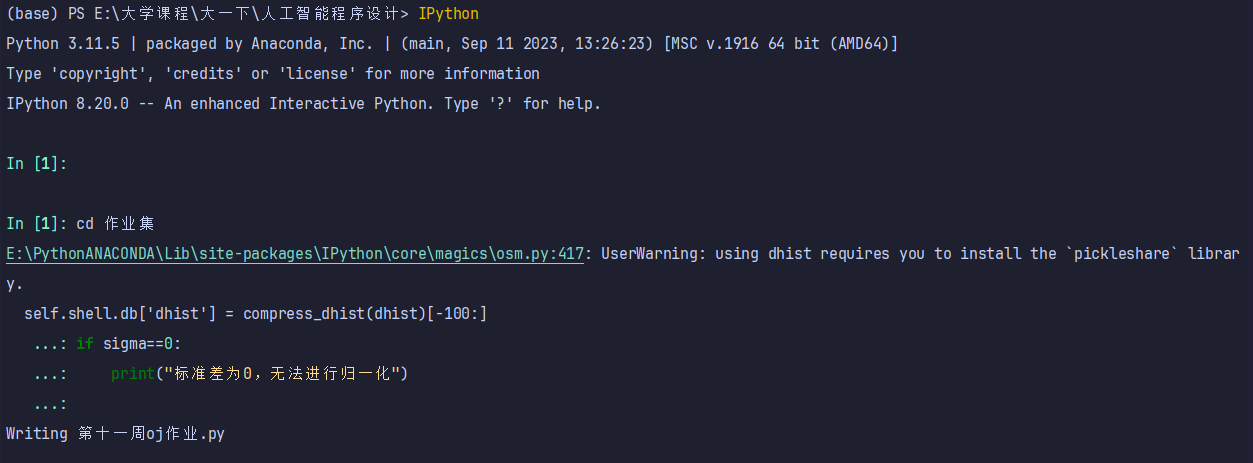
\includegraphics[scale=0.4]{IPython实现矩阵归一化}
		\caption{在IPython中实现矩阵归一化代码}
	\end{figure}
	
	
	\section{Magic Function作用}
	Magic functions是IPython和Jupyter Notebook中的一种特殊命令,
	以百分号\%或者\%\%开头,用于执行与Python代码不同的特定操作,以及控制IPython环境和系统行为等,
	如运行代码、计时、调试和执行系统命令等,这些命令使得在交互式环境中工作更加高效和方便
	\subsection{常用的Magic Function及其作用}
	\subsubsection{\%timeit与\%time作用}
	这两个命令用于测量代码片段的执行时间。它会自动运行多次代码,以得到一个更准确的平均执行时间。这对于性能分析和优化非常有用
	\subsubsection{\%pwd与\%cd与\%ls作用}
	\%pwd用于显示目前运行IPython时所处的文件夹路径\par
	\%cd用于在系统命令行中切换文件夹,比如进入下一级文件夹/返回上一级文件夹\par
	\%ls用于显示目前文件夹下存在的所有文件
	\subsubsection{\%\%writefile命令与\%run命令}
	\%\%writefile命令用于直接编写.py文件的内容并将其保存进.py文件当中
	然后再用\%run命令执行.py文件(此时不用!python命令系统执行)
	
	\section{\%time 和 \%timeit的区别和各自的使用场景}
	\%time 用于简单地测量单次代码执行的时间,输出代码执行的时间和结果
	它适合于快速获取代码执行的近似时间,不需要精确的性能分析。\par
	\%time 只执行一次代码,因此它可能受到系统负载和其他偶然因素的影响,结果可能不够稳定。\par
	\%timeit 用于测量代码的执行时间,它会多次运行代码以计算一个平均时间。
	它自动选择合适的循环次数,以获得更稳定的测量结果,并最终取平均时间并输出,以及执行了多少次循环\par
	\%timeit 适合于需要进行精确性能分析的场景,尤其是需要优化代码或比较不同代码片段的性能时\par
	如果只需要一个快速的估计,可以使用 \%time。
	如果需要进行更精确的性能分析,尤其是对于执行时间很短的代码片段,应该使用 \%timeit\par
	
	
	
	
	\section{NumPy数组在存储和内存使用上的优势}
	\subsection{内存连续性}NumPy 数组在内存中是连续存储的,这意味着数组中的元素都紧密地排列在一起。
	这种存储方式允许 NumPy 快速地进行元素访问和迭代,因为数组中的元素可以通过简单的数学运算来定位。
	而 Python 列表是动态的,它们在内存中可能是非连续的,因此访问和迭代可能需要更复杂的操作。
	\subsection{固定类型}NumPy 数组是同质的,即它们只能存储一种类型的元素(例如,只能是整数或浮点数)\par
	这种类型的一致性允许 NumPy 在内存中更高效地存储数组,因为不需要为每个元素存储额外的类型信息。\par
	相比之下,Python 列表可以包含不同类型的元素,这使得它们在内存中更加灵活但效率较低。
	\subsection{向量化操作}NumPy 数组支持向量化操作,这意味着可以对整个数组或数组的切片执行操作,而不需要显式循环。这些操作通常由底层 C 或 Fortran 代码实现,因此速度比 Python 循环快得多。\par
	而 Python 列表不支持向量化操作,需要使用 Python 循环来实现相同的功能,这通常会更慢。
	\subsection{内存使用效率}由于 NumPy 数组的内存连续性和固定类型,它们通常比 Python 列表更节省内存。\par
	就类似于C++中的struct数组类型会进行数据内存的对齐导致很多内存的浪费,而在NumPy当中由于元素类型是一样的因此可以大大节省内存
	\subsection{并行处理和向量化}NumPy 数组的存储和处理方式使其易于与并行处理库(如 OpenMP)集成,以及利用现代 CPU 的 SIMD(单指令多数据)功能,使得 NumPy 数组在执行大规模数值计算时非常高效。
	
	
	
	\section{\%debug这个Magic Function的功能以及使用方式}
	\subsection{\%debug功能}
	\%debug 是 Jupyter Notebook 中的一个Magic Function,它启动一个交互式调试器,允许用户在代码执行出错时深入检查和调试代码。\par
	在 Jupyter Notebook 中运行代码时,如果遇到错误,使用 \%debug 可以进入调试模式。\par
	在这种模式下,你可以查看变量的值、执行单步执行、检查调用栈、设置断点等,从而帮助你理解代码的行为并找出问题所在。
	\subsection{使用方式}
	1. 打开JupyterNotebook并启用一个.ipynb文件开始写代码\par
	2. 在一个cell中写好代码之后运行发现出错\par
	3. 在下一个cell中写入\%debug,会跳出ipdb(带有提示符的交互式环境)在其中输交互即可\par
	4. 在这个环境中,你可以使用多种命令来调试代码,例如:\\
	p <variable>:打印变量的值\\
	n:执行下一行代码\\
	s:进入当前行的函数或方法\\
	c:继续执行代码直到下一个断点或异常\\
	q:退出调试器\\
	l:列出当前行的代码及其周围代码\\
	b <line>:在指定行设置断点\\
	cl:清除所有断点\\
	disable <breakpoint>:禁用指定的断点\\
	enable <breakpoint>:启用指定的断点\\
	\begin{figure}[H]
		\centering
		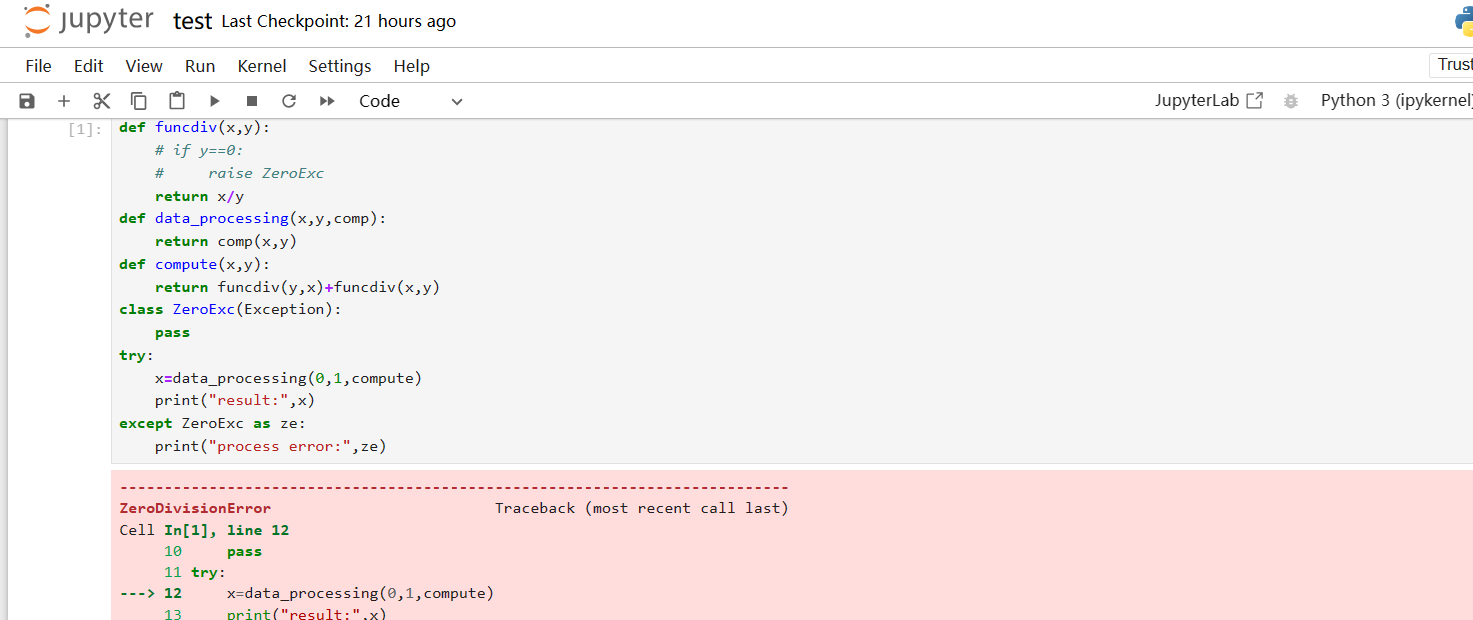
\includegraphics[scale=0.4]{debug}
		\caption{在Jupyter中出现报错}
	\end{figure}
	\begin{figure}[H]
		\centering
		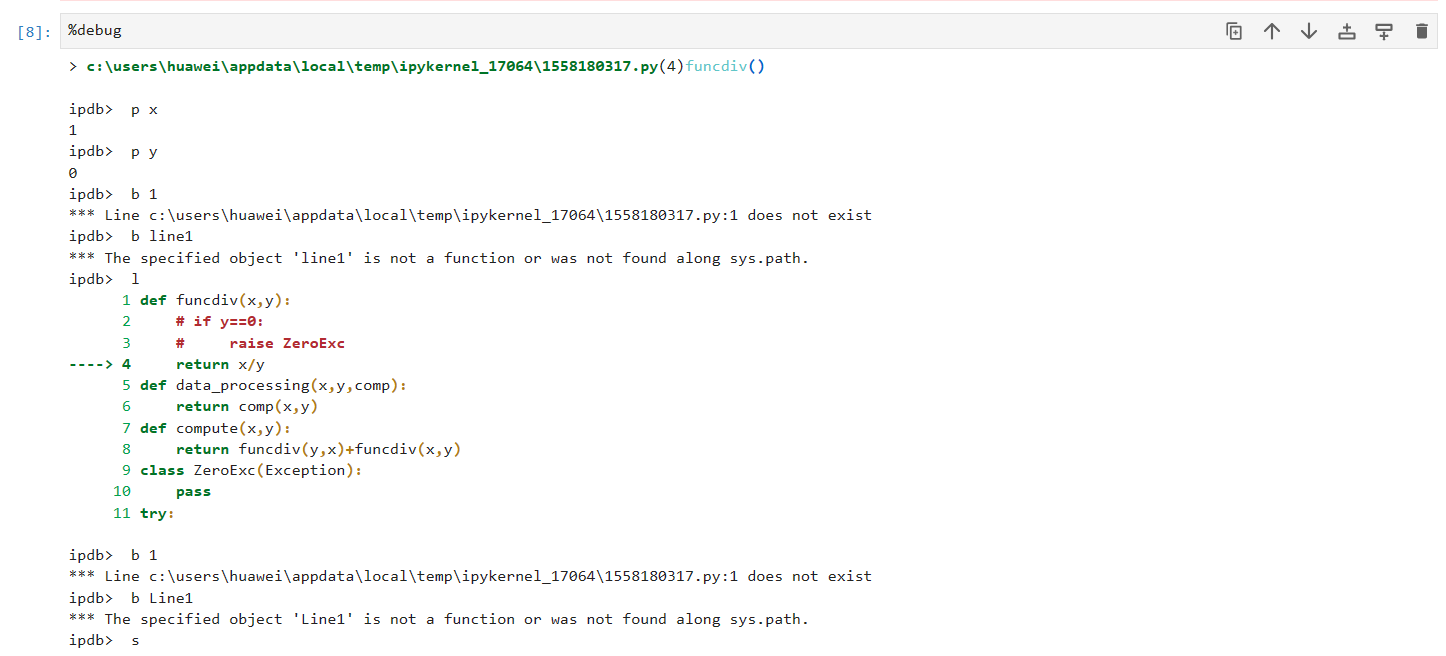
\includegraphics[scale=0.4]{debug1}
		\caption{在Jupyter当中使用\%debug模式}
	\end{figure}
	
	\section{NumPy如何处理和存储高维数组}
	在内部,NumPy 数组(np.ndarray方式)是通过一个称为“数据缓冲区”的连续内存块来存储的,
	这种存储方式允许 NumPy 高效地处理和操作大量数据\par
	NumPy最终仍旧是将一整块高维数组展平成一条一维数组,通过传入strides(n1,n2,……)
	通过n1,n2,……的值来记录需要访问高维数组中某个元素的时候x1,x2,……各自需要跳转多少个字节\par
	这就可以使得当需要数组进行转置的时候不需要对内存块进行复制转移,
	可以直接通过对strides修改从而改变其访问方式就可以实现对数组的转置,实际内部存储方式并未发生改变,极大提高了效率\par
	另外,NumPy还可以通过向量化操作、广播(自动扩展较小的数组与较大数组的形状匹配,从而允许不同形状的数组算术运算)
	以及并行处理等方式提升高维数组计算的效率
	
	
	
	
	\section{NumPy进行数据操作的优点}
	\subsection{性能优化}NumPy的底层使用C语言编写,这使得它在执行数组运算时非常快速。NumPy的数组操作经过高度优化,可以利用底层硬件的并行性,比如SIMD指令集。
	\subsection{丰富的函数库}NumPy包含了大量的数学函数,涵盖了线性代数、概率统计、傅里叶变换等多个数学领域,这些函数可以无缝地在NumPy数组上工作。
	\subsection{广播(Broadcasting)}NumPy的广播机制允许用户在不同大小的数组之间进行算术运算,这在处理数组运算时非常强大且节省时间。
	\subsection{兼容性}NumPy是许多其他科学计算和数据分析库的基础,如SciPy、Pandas、Matplotlib、Scikit-learn等,这使得NumPy成为了Python科学计算生态系统的核心。
	\subsection{跨平台}NumPy可以在多种操作系统上运行,包括Windows、macOS和Linux,可用性和灵活性更高,应用生态更好
	\subsection{社区支持}NumPy拥有一个活跃的社区,不断有新的功能和改进被加入,同时,社区也为用户遇到的各种问题提供了丰富的文档和支持。
	\subsection{适用于大规模数据}尽管NumPy在处理非常大规模的数据集时可能会受到内存限制,但它仍然提供了有效的数据分块和操作机制,使得用户能够处理比内存中能容纳的更大的数据集。 由于这些优点,NumPy成为了数据科学、机器学习以及更广泛的科学计算领域中不可或缺的工具。
	
	
	\section{讨论不同类型的Magic Function}
	\subsection{行magic(line)和单元格magic(cell)}
	行magic一般执行的是一行的命令,用\%开头命令;单元格magic一般执行的是一整块的代码命令,用\%\%开头\par
	比如说要测试代码运行时间性能,\%timeit [i*10 for i in range(10000)]就是行magic执行的是一条语句的时长\par
	而\%\%timeit for i in range(10000):print(i*10)就是cell magic执行一整块的代码
	\subsection{别名magic、模块库magic、系统命令magic}
	别名magic指的是那些允许用户为常用的命令或代码片段定义别名的命令,以便于快速访问。例如,\%alias 用于定义别名。\par
	实用magic命令提供了一些实用的功能,如 \%matplotlib 用于集成 Matplotlib 图形库,\%load 用于加载外部脚本。\par
	系统命令magic允许用户在笔记本中执行系统命令。!开头的命令将被解析为调用系统shell命令,比如!pwd、!cd等等\par
	
	
	\section{借用NumPy思想实现N维矩阵类}
	\begin{figure}[H]
		\centering
		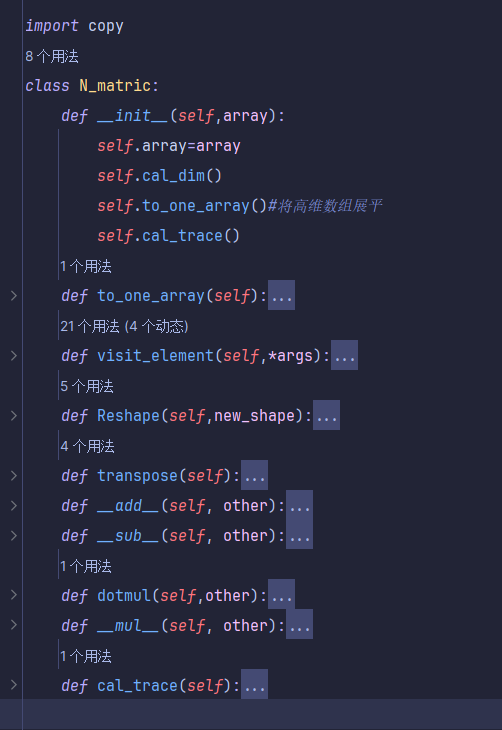
\includegraphics[scale=1.1]{框架}
		\caption{N维矩阵类的框架}
	\end{figure}
		\begin{figure}[H]
		\centering
		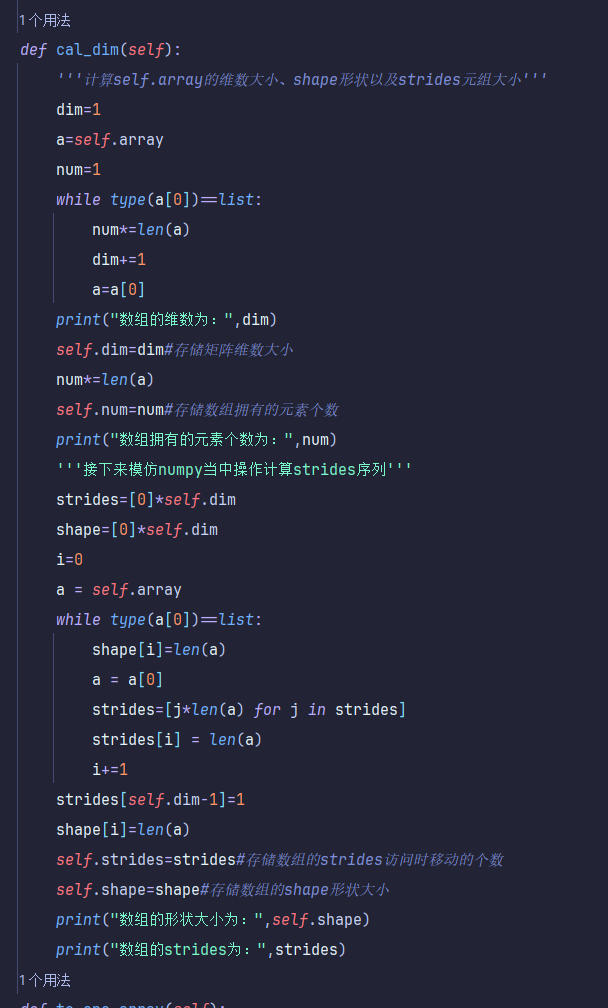
\includegraphics[scale=1]{维度}
		\caption{类中计算数组维度、形状以及strides大小}
	\end{figure}
		\begin{figure}[H]
		\centering
		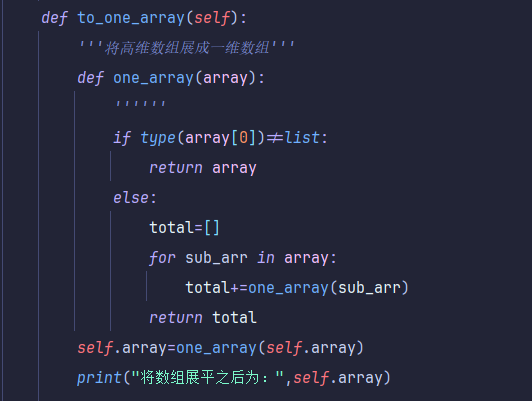
\includegraphics[scale=1.1]{一维}
		\caption{将高维数组展平成一维数组}
	\end{figure}
		\begin{figure}[H]
		\centering
		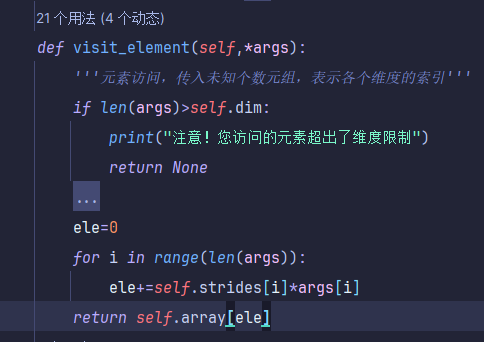
\includegraphics[scale=1]{访问}
		\caption{利用strides访问数组元素}
	\end{figure}
	\begin{figure}[H]
		\centering
		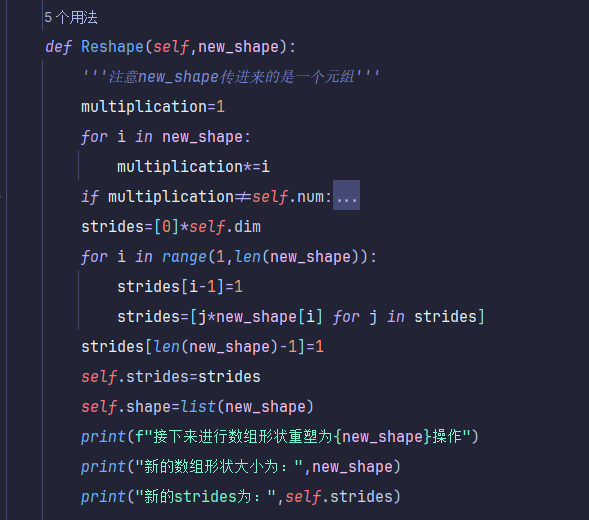
\includegraphics[scale=1]{重塑}
		\caption{类的Reshape方法重塑数组形状}
	\end{figure}
		\begin{figure}[H]
		\centering
		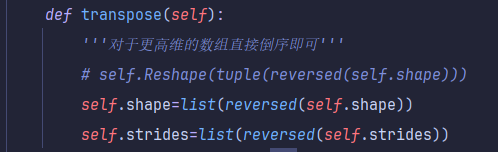
\includegraphics[scale=1]{转置}
		\caption{类的转置transpose方法改变访问方式}
	\end{figure}
		\begin{figure}[H]
		\centering
		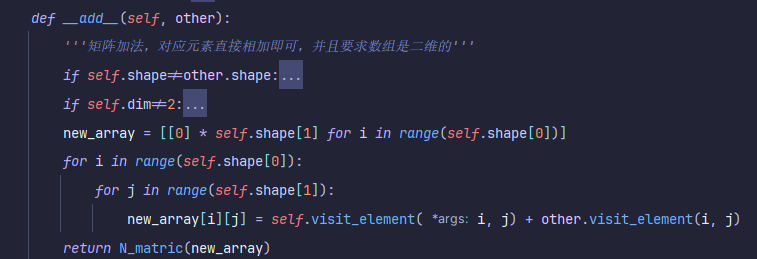
\includegraphics[scale=0.7]{加法}
		\caption{操作符重载实现多维数组直接相加}
	\end{figure}
	\begin{figure}[H]
		\centering
		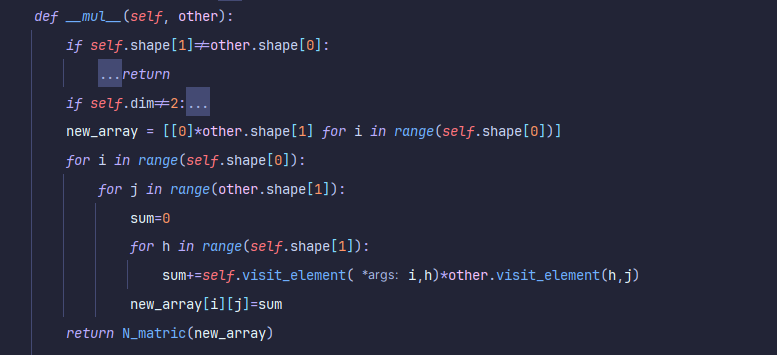
\includegraphics[scale=0.7]{矩阵乘法}
		\caption{操作符重载实现矩阵之间的乘法}
	\end{figure}
	\begin{figure}[H]
		\centering
		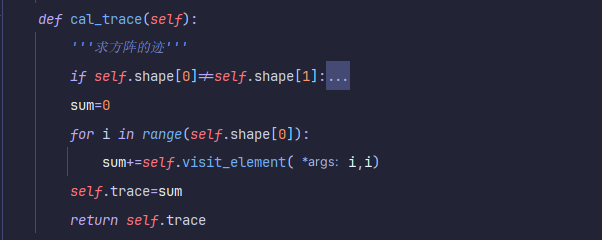
\includegraphics[scale=1]{迹}
		\caption{计算矩阵的迹(主对角线元素之和)}
	\end{figure}
	\begin{figure}[H]
		\centering
		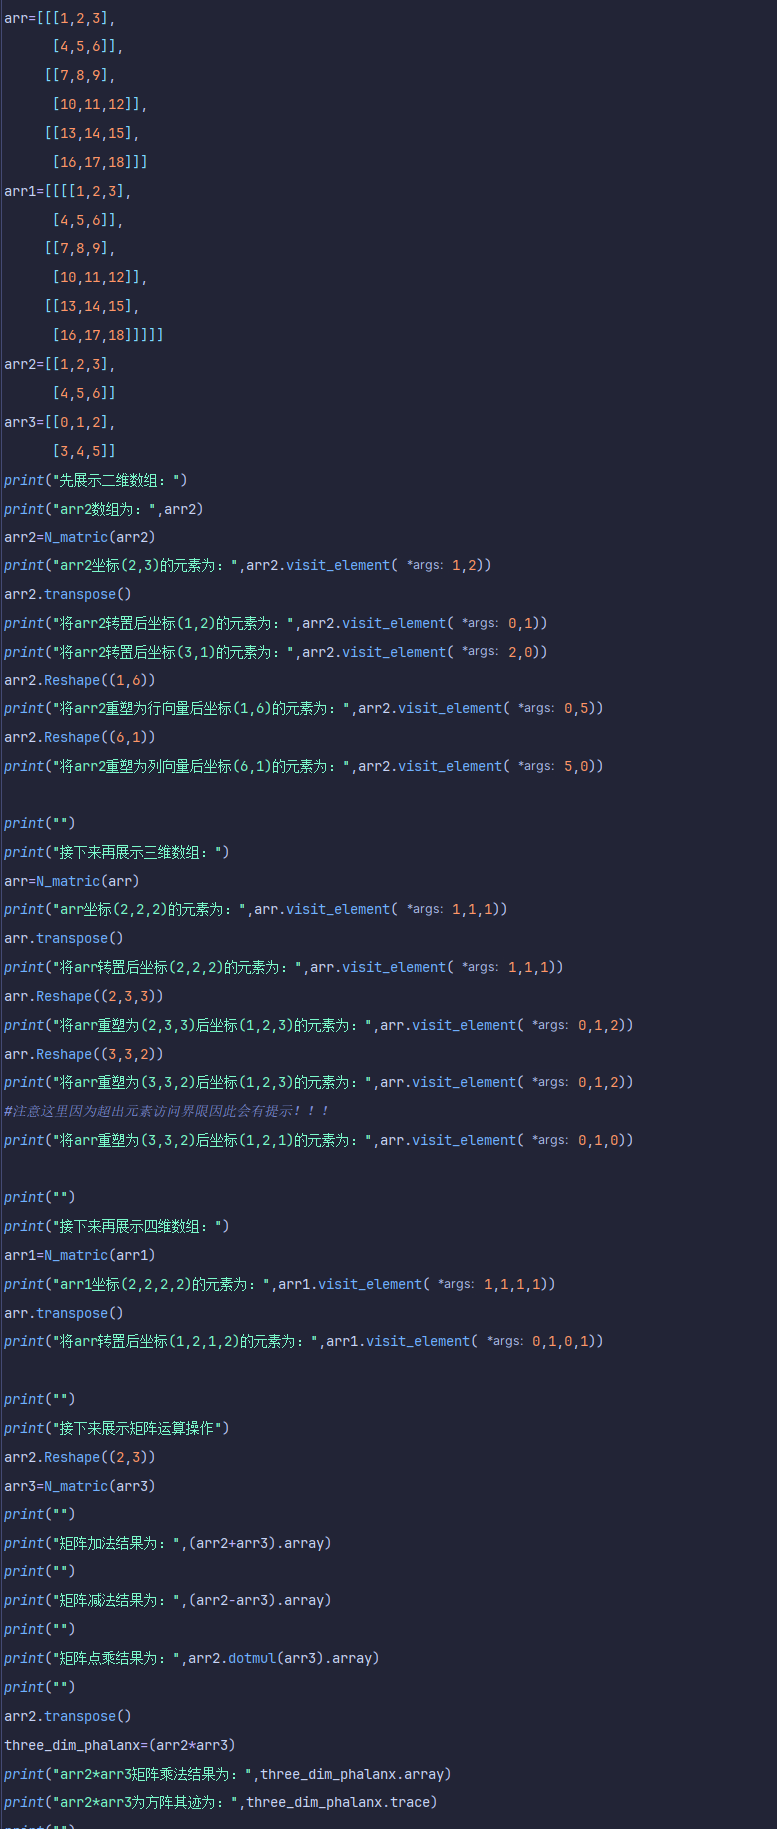
\includegraphics[scale=0.47]{检查}
		\caption{人为编写一些测试数据}
	\end{figure}
	\begin{figure}[H]
		\centering
		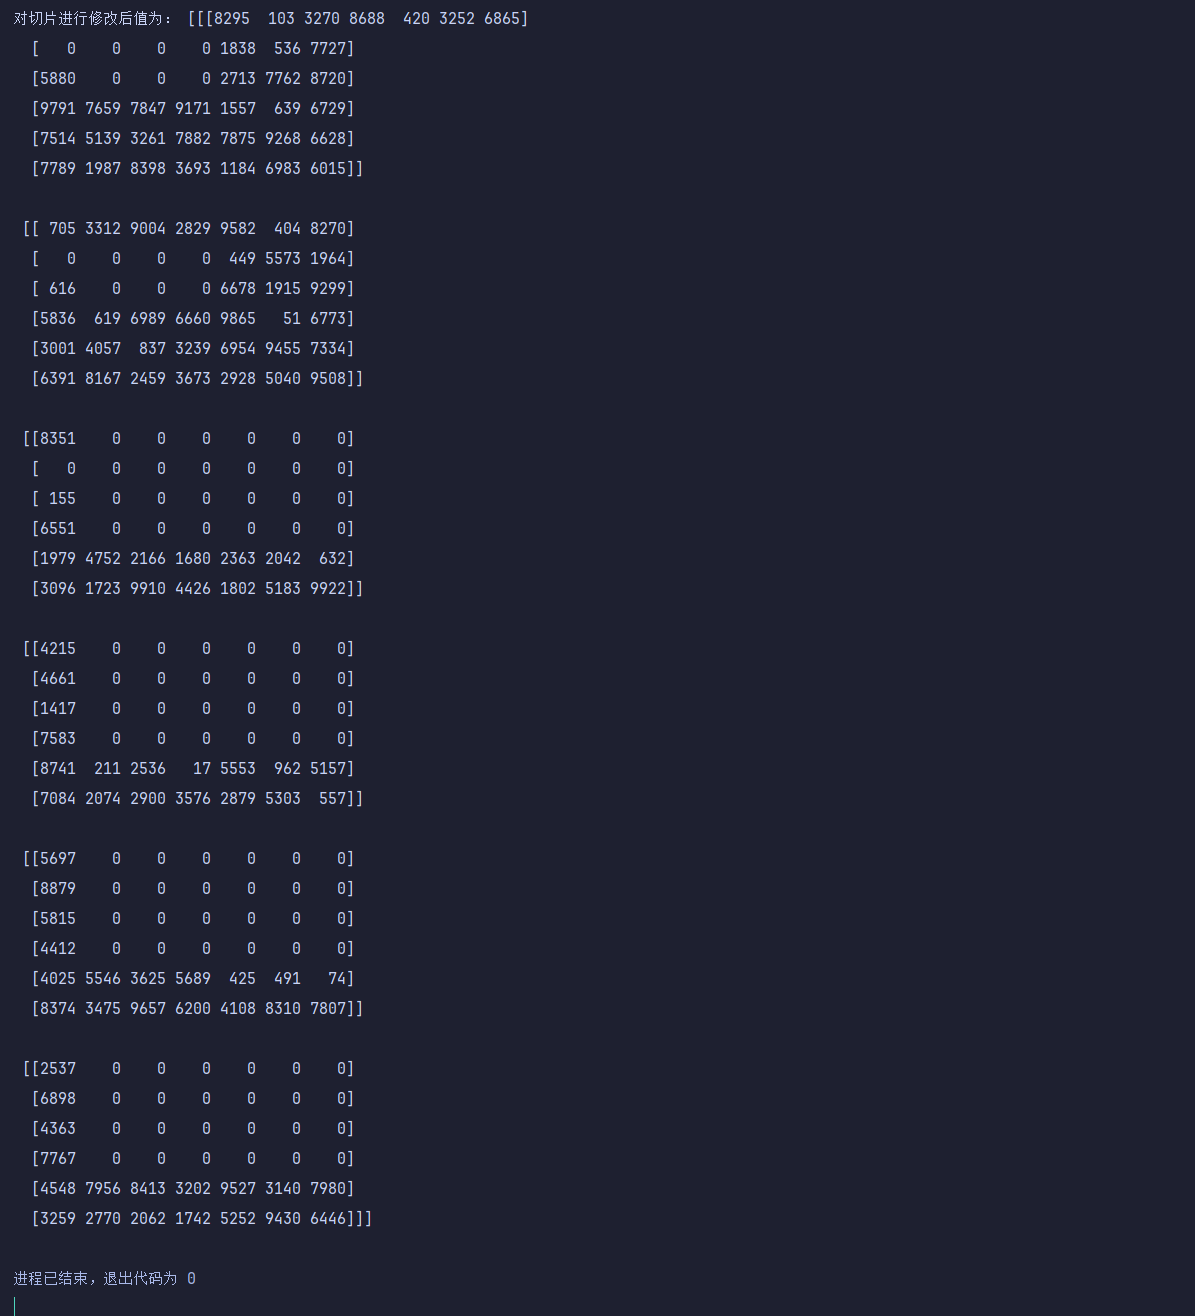
\includegraphics[scale=0.28]{结果}
		\caption{最终运行测试数据结果}
	\end{figure}
\end{document}